Having shown that noise overfitting aligns with increasing  Dirichlet energy and that $E^{dir}$ decreasing methods improve robustness, we now explore an alternative path; a robust loss function. We introduce Graph Centroid Outlier Discounting \method, adapted from \citet{wani2023combining} image classification for learning with noisy labels. Unlike previous methods, \method enhances robustness directly through its formulation, not by explicitly controlling $E^{dir}$
While \method is not designed to directly minimize Dirichlet energy, we investigate its performance in the presence of label noise and, crucially, observe the corresponding behavior in terms of $E^{dir}$.  In this section, we focus on research questions: \textbf{RQ3}.\textit{ Is \method able to prevent learning of noisy samples and promote smoothness of \eqref{eq: avg_dirichlet}, even though it is not specifically designed for it?}
% \textcolor{red}{DO WE NEED THIS SENTENCE?}
% To explain our loss function, we will demonstrate its operation on a single batch of data 
% $\mathcal{B}$ of size $B$. 
% The KL divergence in $L_3$ regulates the alignment of model predictions with the true class for clean samples (small $u$), while preventing alignment for noisy samples (large $u$). The updates for $\theta$ and $u$ are as follows:
We analyze this question through a set of experiments.

 NCOD \citet{wani2023combining} is a loss function designed to address overfitting due to noisy labels for image classification \citep{memorizenoise}. 
%Given its task-agnostic nature, we adopt it for graph classification. 
NCOD assumes samples of the same class are closer in latent space and leverages Deep Neural Networks' tendency to first learn from clean samples before noisy ones \citep{arpit2017closer}. 
%It introduces trainable parameters $\mathbf{u} \in [0, 1]^ n$ (one for each sample), initialized at zero, which increase as the model attempts to memorize noisy samples, and reinforces class centroid representations \cite{wani2023combining}. 


 
 % We introduce the KL divergence term in $\mathcal{L}_3$  with the following two distributions as arguments. One distribution represents the $1-u$ values for samples in the batch, indicating the degree of cleanliness of each sample. For clean samples, the learnable parameter $u$ is small, while it starts to grow for noisy samples, but remains small for clean ones. The other distribution represents the model's prediction score for the class assigned to samples in the dataset. By leveraging the parameter $u$, our objective is to ensure that samples with small $u$ have model prediction aligned with the corresponding class in the dataset while avoiding alignment between samples considered noisy (with large $u$) and their respective classes in the dataset.

% We introduce the KL divergence term in $\mathcal{L}_3$ using two distributions: $\sigma\left(-\log\left(\mathbf{u}_B\right)\right)$ and $\mathfrak{L}$. The first distribution, $\sigma\left(-\log\left(\mathbf{u}_B\right)\right)$, reflects the cleanliness of the samples as clean samples have small $u$ values, while noisy samples exhibit larger $u$. The second distribution, $\mathfrak{L}$, depends on the model's prediction scores for the assigned class. Our goal is to align model predictions with the correct class for clean samples (small $u$) while preventing alignment for noisy samples (large $u$).


 
Our \method method adapts the NCOD framework for graph classification with noisy labels. All the details about the newly designed loss are relegated to Section \ref{appendix:details_GCOD_method} in the Appendix. We introduce two main modifications over the original NCOD.
We add a third loss term $\mathcal{L}_3$ (see eq. \eqref{eq: eq_L3}  in Section \ref{appendix:details_GCOD_method}). This term uses a regularization based on a per sample trainable parameter to help the model distinguish between clean and noisy samples for better alignment.
We incorporate the current training accuracy ($a_{ 
train}$) as feedback into other loss terms (eq \eqref{eq: eq_L1}, \ref{eq: eq_L2} in Section \ref{appendix:details_GCOD_method}). This prioritizes learning from samples that the model correctly fits in early training, assuming these are more likely to be clean.


\method consistently reduces overfitting on noisy samples and preserves smoothness in graph learning, as evidenced by the decreasing Dirichlet energy (Fig. \ref{fig:PPA_DE_NCOD_subfig1} and \ref{fig:PPA_NCOD_Dirich_energy}). Our results for Graph Isomorphism Networks (GIN) \citet{WL1} in Table \ref{tab:ppa_30_perc_6_classes}, Table \ref{tab:alldataset}, and (Fig. \ref{fig:gin_enzymes} and for Graph Convolutional Networks (GCN)  \citet{gcn} in Fig. \ref{fig:NCOD_accuracy} in the Appendix) show that GCOD effectively mitigates noise impact, validating our hypothesis and answering \textbf{RQ3}.


% \begin{table}[htbp]
% \caption{ Performance on the PPA dataset using 30\% of data from 6 selected classes. The best loss function (test accuracy) is highlighted in \textbf{\textcolor{red}{red and bold}}, and the second-best in \textcolor{blue}{blue}. Results show mean $\pm$ standard deviation over 4 runs.
%  }
%     \label{tab:ppa_30_perc_6_classes}
%     \centering
%     %\setlength\extrarowheight{4pt}
%      \renewcommand{\arraystretch}{1.2} %default value 1
%     \resizebox{0.5\textwidth}{!}{
%     \begin{tabular}{c c c c c c }
%         \toprule
%         %\rowcolor{white}
%            \textbf{Noise}  & \textbf{Method} &  \multicolumn{2}{c}{\textbf{Test Accuracy}} & \multicolumn{2}{c }{\textbf{Train Accuracy}}  \\ 
%            \cline{3-6}
%          &  &   \textbf{Best} & \textbf{Last} & \textbf{Best} & \textbf{Last} \\
%          \hline
%         %\rowcolor{white}
%         %\multirow{3}{*}{\rotatebox[origin=c]{90}{\shortstack{  0 \% }}}
%        \multirow{3}{*}{0\% } &   CE &     96.25 $\pm$ 0.05& 91.25 &  1  & 99.33 \\ 
%        &  \method &  96.65 $ \pm$ 0.52& 93.25 & 99.23 & 99.03  \\
%         &  CE+ W2 &     96.50 $ \pm$ 1.12 & 86.5  & 99.76 & 99.29 \\
%         \hline
%         \hline
%        \multirow{5}{*}{20\% }  &  CE   \textcolor{gray}{clean only}&    \textcolor{gray}{96.15 $ \pm$+.09} &  \textcolor{gray}{90.66 }  &  \textcolor{gray}{84.50} &  \textcolor{gray}{84.07} \\
%        \cline{3-6} 
%         &  CE &     88.66 $ \pm$0.16 & 62.58  & 94.98 & 93.45 \\ 
%         & \textcolor{blue}{SOP} &    \textcolor{blue}{91.01 $ \pm$ 0.44} & \textcolor{blue}{85.50 }  & \textcolor{blue}{79.17 } & \textcolor{blue}{77.64 } \\
%          & \textcolor{red}{\method} & \textbf{\textcolor{red}{93.91 $ \pm$ 0.26}} & \textbf{\textcolor{red}{92.58}} & \textcolor{red}{80.11} & \textcolor{red}{79.52 } \\ 
%         & CE + W2&       89.83 $ \pm$ 1.23 & 76.66  & 84.90 & 83.68 \\
%         \hline \hline
%          \multirow{5}{*}{40\% }  &  CE  \textcolor{gray}{clean only}  &   \textcolor{gray}{95.08 $ \pm$ 0.13} &  \textcolor{gray}{80.44} &  \textcolor{gray}{68.15 } &  \textcolor{gray}{67.05}\\
%          \cline{3-6} 
%        &   CE &      82.08 $ \pm$ 0.22 & 51.83  & 82.47 & 78.88  \\ 
%        &   SOP &     82.33 $ \pm$ 1.32  & 65.41    & 58.90  & 57.68 \\ 
%        &  \textcolor{red}{\method} &    \textbf{\textcolor{red}{93.88 $ \pm$ 0.04}} & \textbf{\textcolor{red}{91.08}}  & \textcolor{red}{65.09 } & \textcolor{red}{64.31} \\  
%          &  \textcolor{blue}{CE + W2} &      \textcolor{blue}{88.25 $ \pm$ 1.13} & \textcolor{blue}{56.33 }  & \textcolor{blue}{68.78}& \textcolor{blue}{65.88 }\\ 
%         \bottomrule
%     \end{tabular}}
%     % \caption{ PPA Dataset.  Number of classes 6. 30 \% of. In red and bold the model that performs the best on test accuracy. In blue the one that performs as the second wrt to test accuracy. The mean and standard deviation are calculated from 4 runs of each. }
%     % \label{tab:ppa_30_perc_6_classes}
% \end{table}


\begin{table}[htbp]
  \centering

  % ==== LEFT: PPA, 30 % of data from 6 classes ====================
  \begin{minipage}{0.55\linewidth}
    \centering
    \caption{Performance on the PPA dataset using 30\% of the data restricted to 6 selected classes. The best test accuracy is highlighted in bold red, the second best in blue. Reported values denote mean ± standard deviation across 4 independent runs}
      % \vspace{1pt}
    \label{tab:ppa_30_perc_6_classes}

    \renewcommand{\arraystretch}{1.2}
    \resizebox{\linewidth}{!}{%
      \begin{tabular}{c c c c c c}
        \toprule
        \textbf{Noise} & \textbf{Method} &
        \multicolumn{2}{c}{\textbf{Test Acc.}} &
        \multicolumn{2}{c}{\textbf{Train Acc.}} \\
        \cline{3-6}
        & & \textbf{Best} & \textbf{Last} & \textbf{Best} & \textbf{Last} \\
        \midrule

        % ------------ 0 % noise -------------
        \multirow{5}{*}{0 \%}
          & CE              & 96.25 ± 0.05 & 91.25 &  1.00 & 99.33 \\
          & \method         & 96.65 ± 0.52 & 93.25 & 99.23 & 99.03 \\
          & CE + W2         & 96.50 ± 1.12 & 86.50 & 99.76 & 99.29 \\
          & Fixed           & 96.58 ± 0.27 & 85.70 & 99.26 & 98.29 \\
          & Class-specific  & 96.96 ± 0.04 & 88.67 & 99.41 & 98.67 \\
        \midrule

        % ------------ 20 % noise ------------
        \multirow{7}{*}{20 \%}
          & CE (clean only) & \textcolor{gray}{96.15 ± 0.09} & \textcolor{gray}{90.66}
                            & \textcolor{gray}{84.50} & \textcolor{gray}{84.07} \\ \cline{3-6}
          & CE              & 88.66 ± 0.16 & 62.58 & 94.98 & 93.45 \\
          & SOP             & 91.01 ± 0.44 & 85.50 & 79.17 & 77.64 \\
          & \textcolor{red}{\method}
                            & \textbf{\textcolor{red}{93.91 ± 0.26}} &
                              \textbf{\textcolor{red}{92.58}} &
                              \textcolor{red}{80.11} & \textcolor{red}{79.52} \\
          & CE + W2         & 89.83 ± 1.23 & 76.66 & 84.90 & 83.68 \\
          & Fixed           & 89.69 ± 0.57 & 80.25 & 78.07 & 70.14 \\
          & \textcolor{blue}{Class-specific}$^\ast$
                            & \textcolor{blue}{92.34 ± 0.41} &
                              \textcolor{blue}{80.92} &
                              \textcolor{blue}{84.55} & \textcolor{blue}{83.73} \\
        \midrule

        % ------------ 40 % noise ------------
        \multirow{7}{*}{40 \%}
          & CE (clean only) & \textcolor{gray}{95.08 ± 0.13} & \textcolor{gray}{80.44}
                            & \textcolor{gray}{68.15} & \textcolor{gray}{67.05} \\ \cline{3-6}
          & CE              & 82.08 ± 0.22 & 51.83 & 82.47 & 78.88 \\
          & SOP             & 82.33 ± 1.32 & 65.41 & 58.90 & 57.68 \\
          & \textcolor{red}{\method}
                            & \textbf{\textcolor{red}{93.88 ± 0.04}} &
                              \textbf{\textcolor{red}{91.08}} &
                              \textcolor{red}{65.09} & \textcolor{red}{64.31} \\
          & CE + W2         & 88.25 ± 1.13 & 56.33 & 68.78 & 65.88 \\
          & \textcolor{blue}{Fixed}
                            & \textcolor{blue}{88.58 ± 0.75} &
                              \textcolor{blue}{77.12} &
                              \textcolor{blue}{61.08} & \textcolor{blue}{54.53} \\
          & Class-specific$^\ast$
                            & 88.55 ± 0.11 & 71.83 & 68.98 & 67.80 \\
        \bottomrule
      \end{tabular}%
    }
    \footnotetext{$^\ast$ \small Requires clean validation set.}
  \end{minipage}%
  \hfill
  % ==== RIGHT: 20 % symmetric noise across datasets ===============
  \begin{minipage}{0.42\linewidth}
 
    \caption{Performance of the GIN network across multiple datasets under 40\% asymmetric label noise. Reported values are test accuracy (\%). Columns correspond to cross-entropy (CE) with clean labels (0\% CE), cross entropy with noisy labels (40\% CE), and GCOD under 40\% noise (40\% GCOD).}
    \label{tab:asymmetric_noise}
     \resizebox{\linewidth}{!}{\begin{tabular}{lccc}
      \hline
      \textbf{Dataset} & \textbf{0\% CE} & \textbf{40\% CE} & \textbf{40\% GCOD} \\ \hline
      PROTEINS & 81.16 & 72.90 & 76.19 \\
      MNIST    & 72.69 & 71.15 & 72.61 \\
      ENZYMES  & 73.33 & 65.80 & 69.81 \\
      IMDB/B   & 76.50 & 68.18 & 72.89 \\
      MUTAG    & 94.73 & 91.16 & 93.19 \\
      REDDIT   & 48.15 & 48.01 & 47.94 \\
      MSRC/21  & 96.69 & 94.39 & 95.57 \\ \hline
    \end{tabular}}
\vspace{25pt}
     \centering
    \caption{Percentage improvement over cross entropy (CE) using the GIN network. Values show gains of OMG and GCOD on selected datasets.}
    \label{tab:omg_table}
    \begin{tabular}{lcc}
      \hline
      \textbf{Dataset} & \textbf{OMG} & \textbf{GCOD} \\ \hline
      MUTAG    & 0.061 & 0.062 \\
      IMDB-B   & 0.047 & 0.049 \\
      PROTEINS & 0.039 & 0.041 \\ \hline
    \end{tabular}    
\end{minipage}

\end{table}


% \begin{table}[htbp]
% \caption{Performance on the PPA dataset using 30\% of data from 6 selected classes. The best method (test accuracy) is highlighted in \textbf{\textcolor{red}{red and bold}}, and the second-best in \textcolor{blue}{blue}. Results show mean $\pm$ standard deviation over 4 runs.
%  }
%     \label{tab:ppa_30_perc_6_classes}
%     \centering
%     %\setlength\extrarowheight{4pt}
%      \renewcommand{\arraystretch}{1.2} %default value 1
%     \resizebox{0.5\textwidth}{!}{
%     \begin{tabular}{c c c c c c }
%         \toprule
%         %\rowcolor{white}
%         \textbf{Noise}  & \textbf{Method} &  \multicolumn{2}{c}{\textbf{Test Accuracy}} & \multicolumn{2}{c }{\textbf{Train Accuracy}}  \\ 
%         \cline{3-6}
%          &  & \textbf{Best} & \textbf{Last} & \textbf{Best} & \textbf{Last} \\
%          \hline
         
%         %\rowcolor{white}
%         %\multirow{3}{*}{\rotatebox[origin=c]{90}{\shortstack{  0 \% }}}

        
%         \multirow{5}{*}{0\% } 
%         &   CE &     96.25 $\pm$ 0.05& 91.25 &  1  & 99.33 \\ 
%         &  \method &  96.65 $ \pm$ 0.52& 93.25 & 99.23 & 99.03  \\
%         &  CE+ W2 &     96.50 $ \pm$ 1.12 & 86.5  & 99.76 & 99.29 \\ 
%         & Fixed & 96.58 $\pm$ 0.27 & 85.70 & 99.26  & 98.29  \\
%         & Class-specific$^*$ & 96.96 $\pm$ 0.04 & 88.67 & 99.41 & 98.67 \\
%         \hline
%         \hline
        
%         \multirow{7}{*}{20\% }  
%         &  CE   \textcolor{gray}{clean only}&    \textcolor{gray}{96.15 $ \pm$+.09} &  \textcolor{gray}{90.66 }  &  \textcolor{gray}{84.50} &  \textcolor{gray}{84.07} \\
%         \cline{3-6} 
%         &  CE &   88.66 $\pm$0.16 & 62.58  & 94.98 & 93.45 \\ 
%         &  SOP &   91.01 $\pm$ 0.44 & 85.50 & 79.17 &  77.64 \\
%         & \textcolor{red}{\method} & \textbf{\textcolor{red}{93.91 $\pm$ 0.26}} & \textbf{\textcolor{red}{92.58}} & \textcolor{red}{80.11} & \textcolor{red}{79.52} \\ 
%         & CE + W2 &  89.83 $\pm$ 1.23 & 76.66  & 84.90 & 83.68 \\
%         & Fixed & 89.69 $\pm $0.57 & 80.25 & 78.07 & 70.14  \\
%         & \textcolor{blue}{Class-specific}$^*$ & \textcolor{blue}{92.34 $\pm$ 0.41} & \textcolor{blue}{80.92} & \textcolor{blue}{84.55}  & \textcolor{blue}{83.73}  \\
%         \hline \hline


        
%         \multirow{7}{*}{40\% }  &  CE  \textcolor{gray}{clean only}  &   \textcolor{gray}{95.08 $ \pm$ 0.13} &  \textcolor{gray}{80.44} &  \textcolor{gray}{68.15 } &  \textcolor{gray}{67.05}\\
%         \cline{3-6} 
%         &   CE &      82.08 $ \pm$ 0.22 & 51.83  & 82.47 & 78.88  \\ 
%         &   SOP &     82.33 $ \pm$ 1.32  & 65.41    & 58.90  & 57.68 \\ 
%         &  \textcolor{red}{\method} &    \textbf{\textcolor{red}{93.88 $\pm$ 0.04}} & \textbf{\textcolor{red}{91.08}}  & \textcolor{red}{65.09 } & \textcolor{red}{64.31} \\  
%         &  CE + W2 &   88.25 $ \pm$ 1.13 & 56.33  & 68.78 & 65.88 \\ 
%          & \textcolor{blue}{Fixed} & \textcolor{blue}{88.58 $\pm$ 0.75} & \textcolor{blue}{77.12} & \textcolor{blue}{61.08} & \textcolor{blue}{54.53}  \\
%         &  Class-specific$^*$ & 88.55 $\pm$ 0.11& 71.83 & 68.98 & 67.80  \\

%         \bottomrule
%     \end{tabular}
%     }
%     % \caption{ PPA Dataset.  Number of classes 6. 30 \% of. In red and bold the model that performs the best on test accuracy. In blue the one that performs as the second wrt to test accuracy. The mean and standard deviation are calculated from 4 runs of each. }
%     % \label{tab:ppa_30_perc_6_classes}
% \end{table}






% \begin{table}[htbp]
% \caption{Performance comparison of CE and GCOD across datasets with 20\% symmetric label noise for the same model. The last column summarizes the test accuracy difference between GCOD and CE for 20\% noise.}
% \label{tab:alldataset}
% \centering
% \begin{adjustbox}{width=0.47\textwidth}
% \begin{tabular}{llcccc}
% \hline
% \textbf{Dataset}       & \textbf{Metric}   & \textbf{0\% CE} & \textbf{20\% CE} & \textbf{20\% GCOD} & \makecell[c]{20\% \\(GCOD-CE)} \\ \hline
% \multirow{3}{*}{MNIST}       & Best              & 72.69         & 66.30          & 71.26            & +4.96                    \\ 
%                        & Last              & 69.80         & 53.64          & 67.88            & +14.24                   \\ \cline{3-5} 
%                        & Difference        & 2.89          & 12.66          & 3.38             &                   \\ \hline
% \multirow{3}{*}{ENZYMES}      & Best              & 73.33         & 64.16          & 68.69            & +4.53                    \\ 
%                        & Last              & 65.78         & 57.50         & 62.54            & +5.04                    \\ \cline{3-5} 
%                        & Difference        & 7.55          & 6.66           & 6.15            &                    \\ \hline
% \multirow{3}{*}{MSRC\_21}     & Best              & 96.69         & 90.26          & 94.69            & +4.43                    \\
%                        & Last              & 93.80         & 79.64          & 90.26            & +10.62                   \\ \cline{3-5} 
%                        & Difference        & 2.89          & 10.62          & 4.43             &                   \\ \hline
% \multirow{3}{*}{PROTEINS}      & Best              & 81.16         & 76.23          & 79.38            & +3.15                    \\ 
%                        & Last              & 79.18         & 62.32          & 78.12            & +15.80                   \\ \cline{3-5} 
%                        & Difference        & 1.98          & 13.91          & 1.26             &                    \\ \hline
% \multirow{3}{*}{MUTAG}     & Best              & 94.73         & 89.47          & 90.01            & +0.54                    \\
%                        & Last              & 84.21         & 68.42          & 86.84            & +18.42                   \\ \cline{3-5} 
%                        & Difference        & 10.52         & 21.05          & 3.17            &                    \\ \hline
% \multirow{3}{*}{\makecell[l]{IMDB-\\BINARY}}   & Best              & 76.50         & 75.00          & 75.40            & +0.40                    \\ 
%                        & Last              & 71.60         & 71.00          & 73.50            & +2.50                    \\ \cline{3-5} 
%                        & Difference        & 4.90          & 4.00           & 1.90             &                    \\ \hline
% \multirow{3}{*}{\makecell[l]{REDDIT-\\MULTI-12K} }& Best           & 48.15         & 45.05          & 44.98            & -0.07                    \\ 
%                        & Last              & 46.01         & 44.67          & 44.89            & +0.22                    \\ \cline{3-5} 
%                        & Difference        & 2.14          & 0.38           & 0.09             &                    \\ \hline
% \end{tabular}
% \end{adjustbox}
% % \caption{Performance comparison across different datasets for 20\% symmetrical noise. The last column shows the difference between 20\% noise with GCOD and 20\% noise with CE.}
% % \label{tab:alldataset}
% \end{table}










%  \begin{table}[htbp]
% \caption{ Performance on the PPA dataset using 30\% of data from 6 selected classes. The best loss function (test accuracy) is highlighted in \textbf{\textcolor{red}{red and bold}}, and the second-best in \textcolor{blue}{blue}. Results show mean $\pm$ standard deviation over 4 runs.
%  }
%     \label{tab:ppa_30_perc_6_classes}
%     \centering
%     %\setlength\extrarowheight{4pt}
%      \renewcommand{\arraystretch}{1.2} %default value 1
%     \resizebox{0.5\textwidth}{!}{
%     \begin{tabular}{c c c c c c }
%         \toprule
%         %\rowcolor{white}
%            \textbf{Noise}  & \textbf{Method} &  \multicolumn{2}{c}{\textbf{Test Accuracy}} & \multicolumn{2}{c }{\textbf{Train Accuracy}}  \\ 
%            \cline{3-6}
%          &  &   \textbf{Best} & \textbf{Last} & \textbf{Best} & \textbf{Last} \\
%          \hline
%         %\rowcolor{white}
%         %\multirow{3}{*}{\rotatebox[origin=c]{90}{\shortstack{  0 \% }}}
%        \multirow{3}{*}{0\% } &   CE &     96.25 $\pm$ 0.05& 91.25 &  1  & 99.33 \\ 
%        &  \method &  96.65 $ \pm$ 0.52& 93.25 & 99.23 & 99.03  \\
%         &  CE+ W2 &     96.50 $ \pm$ 1.12 & 86.5  & 99.76 & 99.29 \\
%         \hline
%         \hline
%        \multirow{5}{*}{20\% }  &  CE   \textcolor{gray}{clean only}&    \textcolor{gray}{96.15 $ \pm$+.09} &  \textcolor{gray}{90.66 }  &  \textcolor{gray}{84.50} &  \textcolor{gray}{84.07} \\
%        \cline{3-6} 
%         &  CE &     88.66 $ \pm$0.16 & 62.58  & 94.98 & 93.45 \\ 
%         & \textcolor{blue}{SOP} &    \textcolor{blue}{91.01 $ \pm$ 0.44} & \textcolor{blue}{85.50 }  & \textcolor{blue}{79.17 } & \textcolor{blue}{77.64 } \\
%          & \textcolor{red}{\method} & \textbf{\textcolor{red}{93.91 $ \pm$ 0.26}} & \textbf{\textcolor{red}{92.58}} & \textcolor{red}{80.11} & \textcolor{red}{79.52 } \\ 
%         & CE + W2&       89.83 $ \pm$ 1.23 & 76.66  & 84.90 & 83.68 \\
%         \hline \hline
%          \multirow{5}{*}{40\% }  &  CE  \textcolor{gray}{clean only}  &   \textcolor{gray}{95.08 $ \pm$ 0.13} &  \textcolor{gray}{80.44} &  \textcolor{gray}{68.15 } &  \textcolor{gray}{67.05}\\
%          \cline{3-6} 
%        &   CE &      82.08 $ \pm$ 0.22 & 51.83  & 82.47 & 78.88  \\ 
%        &   SOP &     82.33 $ \pm$ 1.32  & 65.41    & 58.90  & 57.68 \\ 
%        &  \textcolor{red}{\method} &    \textbf{\textcolor{red}{93.88 $ \pm$ 0.04}} & \textbf{\textcolor{red}{91.08}}  & \textcolor{red}{65.09 } & \textcolor{red}{64.31} \\  
%          &  \textcolor{blue}{CE + W2} &      \textcolor{blue}{88.25 $ \pm$ 1.13} & \textcolor{blue}{56.33 }  & \textcolor{blue}{68.78}& \textcolor{blue}{65.88 }\\ 
%         \bottomrule
%     \end{tabular}}
%     % \caption{ PPA Dataset.  Number of classes 6. 30 \% of. In red and bold the model that performs the best on test accuracy. In blue the one that performs as the second wrt to test accuracy. The mean and standard deviation are calculated from 4 runs of each. }
%     % \label{tab:ppa_30_perc_6_classes}
% \end{table}
% \begin{table}[htbp]
% \caption{Performance comparison of CE and GCOD across datasets with 20\% symmetric label noise for the same model. The last column summarizes the test accuracy difference between GCOD and CE for 20\% noise.}
% \label{tab:alldataset}
% \centering
% \begin{adjustbox}{width=0.47\textwidth}
% \begin{tabular}{llcccc}
% \hline
% \textbf{Dataset}       & \textbf{Metric}   & \textbf{0\% CE} & \textbf{20\% CE} & \textbf{20\% GCOD} & \makecell[c]{20\% \\(GCOD-CE)} \\ \hline
% \multirow{3}{*}{MNIST}       & Best              & 72.69         & 66.30          & 71.26            & +4.96                    \\ 
%                        & Last              & 69.80         & 53.64          & 67.88            & +14.24                   \\ \cline{3-5} 
%                        & Difference        & 2.89          & 12.66          & 3.38             &                   \\ \hline
% \multirow{3}{*}{ENZYMES}      & Best              & 73.33         & 64.16          & 68.69            & +4.53                    \\ 
%                        & Last              & 65.78         & 57.50         & 62.54            & +5.04                    \\ \cline{3-5} 
%                        & Difference        & 7.55          & 6.66           & 6.15            &                    \\ \hline
% \multirow{3}{*}{MSRC\_21}     & Best              & 96.69         & 90.26          & 94.69            & +4.43                    \\
%                        & Last              & 93.80         & 79.64          & 90.26            & +10.62                   \\ \cline{3-5} 
%                        & Difference        & 2.89          & 10.62          & 4.43             &                   \\ \hline
% \multirow{3}{*}{PROTEINS}      & Best              & 81.16         & 76.23          & 79.38            & +3.15                    \\ 
%                        & Last              & 79.18         & 62.32          & 78.12            & +15.80                   \\ \cline{3-5} 
%                        & Difference        & 1.98          & 13.91          & 1.26             &                    \\ \hline
% \multirow{3}{*}{MUTAG}     & Best              & 94.73         & 89.47          & 90.01            & +0.54                    \\
%                        & Last              & 84.21         & 68.42          & 86.84            & +18.42                   \\ \cline{3-5} 
%                        & Difference        & 10.52         & 21.05          & 3.17            &                    \\ \hline
% \multirow{3}{*}{\makecell[l]{IMDB-\\BINARY}}   & Best              & 76.50         & 75.00          & 75.40            & +0.40                    \\ 
%                        & Last              & 71.60         & 71.00          & 73.50            & +2.50                    \\ \cline{3-5} 
%                        & Difference        & 4.90          & 4.00           & 1.90             &                    \\ \hline
% \multirow{3}{*}{\makecell[l]{REDDIT-\\MULTI-12K} }& Best           & 48.15         & 45.05          & 44.98            & -0.07                    \\ 
%                        & Last              & 46.01         & 44.67          & 44.89            & +0.22                    \\ \cline{3-5} 
%                        & Difference        & 2.14          & 0.38           & 0.09             &                    \\ \hline
% \end{tabular}
% \end{adjustbox}
% % \caption{Performance comparison across different datasets for 20\% symmetrical noise. The last column shows the difference between 20\% noise with GCOD and 20\% noise with CE.}
% % \label{tab:alldataset}
% \end{table}
% Our robust loss function consistently observes a trend across all datasets containing noise, there is no evidence of overfitting on noisy samples. This phenomenon remains consistent regardless of the dataset size or the size of the graphs, demonstrating the loss function's ability to promote robust learning in the presence of noise.

% Furthermore, we notice that the total Dirichlet energy of the training set consistently decreases during the training process when employing this loss (see Figure \ref{fig:PPA_DE_NCOD_subfig1} and \ref{fig:PPA_NCOD_Dirich_energy}. This trend aligns with our hypothesis, suggesting that a loss function tailored to learn solely from clean samples, while disregarding noisy signals, prioritizes low-frequency components, thereby enhancing the smoothness of graphs during learning. These findings corroborate our hypothesis presented in the previous section and answer positively to \textbf{RQ3}. Our results, as shown in Table \ref{tab:ppa_30_perc_6_classes}, Table \ref{tab:alldataset}  and Figure \ref{fig:NCOD_accuracy}, demonstrate that the GCOD approach effectively mitigates the impact of noise during training.

%Illustrating this behavior, Figure \ref{fig:NCOD_accuracy}, fig:NCOD_Dirich_energy} and Table \ref{tab: results} present a comprehensive analysis of the performance and dynamics of the loss function across diverse datasets.


%differntnoise_Dirchi_CE_NCOD.png


% \begin{figure}[t!]
%     \centering
%     \begin{subfigure}[b]{0.5\textwidth}
%         \centering
%         %\includegraphics[scale = 0.25]{Neurips/Screenshots/gin_drchi_6Classes_30/20_N_P_drichi.png}
%         %
\includegraphics[page=1,width=1.0\textwidth]{Neurips/figures/fig8a}
%         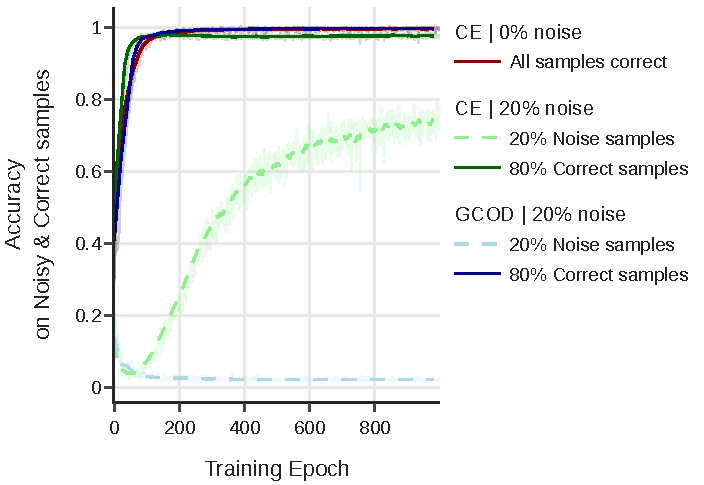
\includegraphics[page=1,width=1.0\textwidth]{AISTATS/figures/fig8a}
%         \caption{Avg. Accuracy for GIN model on the PPA dataset (30\% sample, 6 classes) with clean or 20\% label noise. CE represents Cross Entropy, while \method refers to our modified loss function. 
%         %In particular, we show the average accuracy for three classes ( taken from the 6). For the case with 0\% noise, there are no noisy samples and we reported the accuracy of all samples. For the case of 20\% noise, we reported both the average accuracy of pure samples and the average accuracy of noisy samples.  
%         }
%         \label{fig:PPA_DE_NCOD_subfig1}
%     \end{subfigure}
%        % \vspace{0.5cm}


%     \begin{subfigure}[b]{0.5\textwidth}
%  \centering
%         %\includegraphics[scale = 0.25]{Neurips/Screenshots/gin_drchi_6Classes_30/differntnoise_Dirchi_CE_NCOD.png}
%         %
\includegraphics[page=1,width=1.0\textwidth]{Neurips/figures/fig8b}
%         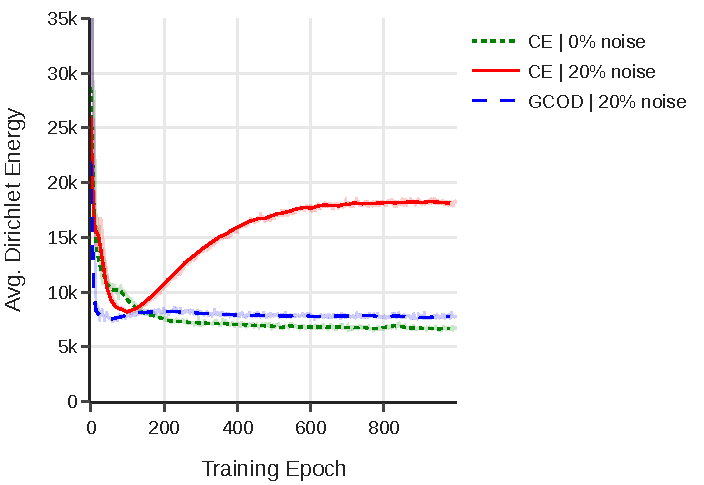
\includegraphics[width=\textwidth]{AISTATS/figures/fig8b}
%         \caption{Evolution of Representation Dirichlet energy for clean and noise-introduced PPA dataset (30\% sample, 6 classes). Dirichlet energy increases, when the model with CrossEntropy fits on noise. }
%         \label{fig:PPA_NCOD_Dirich_energy}
%     \end{subfigure}
%     \caption{}
%     \label{fig:mainfig}
% \end{figure}


% We first normalize each graph representation before the final prediction as $\phi(\mathbf{z}_i) = \frac{\mathbf{z}_i}{\|\mathbf{z}_i\|}$. For each class $c \in C$, its vector representation is the average of the latent representations of its training samples:
% \begin{equation}
% \mathbf{z}_c = \frac{1}{n_c} \sum_{i=1, c_i=c} \mathbf{z}_i,
% \end{equation}

% where \( n_c \) is the number of samples for class \( c \). The class embedding is normalized:

% \begin{equation}
% \label{eq: class_centroid}
% \mathbf{\phi}_c = \frac{\mathbf{z}_c}{\|\mathbf{z}_c\|}.
% \end{equation}

% The soft label \( \mathbf{\tilde{y}}_i \) for sample \( i \) is the similarity between its normalized feature representation $\mathbf{\phi(\mathbf{z}_i)}$ and the class embedding $\mathbf{\phi}_c$:

% \begin{equation}
% \mathbf{\tilde{y}}_i = \left[ \max(\mathbf{\phi(\mathbf{z}_i)} \mathbf{\phi_c}^T, 0) \mathbf{y}_i \right].
% \end{equation}
% More specific details and theoretical proofs on this loss are available in the original paper \cite{wani2023combining}.


% \textbf{Model Capacity and Noise Fitting}
% We conjecture that this issue is related to the capacity of the model. Specifically, the model lacks sufficient capacity to effectively differentiate between clean data and noise. This is evident when we manipulate the dataset by adding classes; for instance, when the number of classes is increased, the model fits noise less and less. Conversely, reducing the dataset size often leads to the model fitting noise more easily.

% \textbf{Role of Dirichlet Energy}
% The concept of Dirichlet energy becomes relevant here. Dirichlet energy can become a metric that can provide insights into the model's 
% \textit{Why do adding classes make the Dirichlet energy of a sample increase?}
% Smoothing is better for graph classification. 

% When additional classes are introduced, the Dirichlet energy of a sample increases if the model has adequate capacity. This suggests that the number of classes directly impacts the Dirichlet energy, which in turn affects the model’s ability to handle noise. An increased number of classes leads to higher Dirichlet energy, reflecting the added complexity and variance due to noise.


% \textbf{Noise and Variance}
% Noise inherently increases variance within the dataset. When multiple noisy samples are aggregated, the overall Dirichlet energy tends to increase, indicating higher variability and complexity that the model must learn to manage.

% \textbf{Observations and Implications}
% Our observations suggest that whenever the model attempts to learn from noise, its performance is adversely affected. 
% This is because noise introduces inconsistencies (like if we are asking the model to put together graphs that have a different structure and it's like we're asking the model to introduce some sharpening instead of only smoothing, this is why the Dirichlet energy increases).



% \textbf{Future Works}

% Incorporating Dirichlet energy into the loss function and ensuring the model has sufficient capacity to handle complex datasets with multiple classes can enhance robustness and accuracy in graph classification tasks.




% \subsection{Introduction of Label Noise: not much difference between  performances obtained by cross entropy and by a robust loss function}

% For the subsequent experiments involving the introduction of label noise into the PPA dataset, we initially introduced 20\% noise. When employing cross-entropy, two noteworthy phenomena emerged. Firstly, the decline in accuracy from the zero noise to the 20\% noise scenario was marginal compared to typical observations in image datasets with different deep neural networks (DNNs) \cite{?}, see also Figure and appendix .. for a more detailed discussion.  Secondly, the accuracy did not display indications of overfitting to noise throughout the continued training with cross-entropy, contrary to conventional expectations.

% The utilization of specific noise robust loss functions such as the one proposed in \cite{wani2023combining} did not lead to significant improvements beyond the performance achieved with cross-entropy. This pattern persisted even with a higher noise level of 40\%, where identical results were obtained, as depicted in \cref{??}
 



% \subsubsection{Simple Cross-Entropy on sufficiently complex data ensures robustness against fitting noisy labels.}

% To understand why a robust loss function yielded similar or only slightly better results compared to cross-entropy, we examined how the GCN model learned from noisy samples in the presence of noisy labels. Surprisingly, we discovered that the model never overfits the noisy samples for such a large and complex dataset. Consequently, we observed no significant improvement over cross-entropy, nor did we experience a substantial decrease in performance compared to the zero-noise scenario (see Figure \ref{noisy_pure_40_1}).

% \subsubsection{A small decrease in accuracy is noticeable}

% Examining the learning behavior of GCN on the PPA dataset in the presence of noise sheds light on why a custom loss function did not lead to any accuracy improvements compared to CE. However, an intriguing question arises: why do we observe a slight decrease in accuracy when noise is introduced? I attribute this decline primarily to the reduction in the number of samples per class, which may cause a minor decrease in accuracy. Perhaps conducting an experiment specifically addressing this aspect would provide further insights.

% \subsubsection{Effectiveness of GIN Network}

% We also posited that perhaps the network is not that strong which might contribute to its inability to overfit on noise. To investigate this further, we replicated our experiments using the GIN network. Surprisingly, even with a stronger network, we observed that the model continued to resist overfitting on noise (see Figure \ref{noisy_pure_40_0}). However, with our loss function, we noticed slight improvements in results (see Figure \ref{test_gin}). It's possible that under cross-entropy, the model fitted a few more noisy samples on average, albeit insignificantly. Additionally, we incorporated the effect of training accuracy into our loss function calculation, resulting in a slightly modified loss function that enhances its robustness for GNN applications.

% \subsubsection{Clusterability Analysis}

% Additionally, we investigated the clusterability of the latent space representation generated by both the GIN and GCN models. We observed that the clusterability of the GIN model is significantly superior to that of the GCN model, which contributes to the improved performance of our loss function. However, the question remains unanswered as to why this powerful network fails to fit noise, despite demonstrating nearly 95\% training accuracy under zero noise conditions.

% \subsubsection{Encountered fitting on Noise}


% Subsequently, as we did not encounter overfitting with larger datasets containing many nodes per class, we shifted our analysis to smaller datasets with fewer nodes per graph. During this process, we observed that the model tends to fit the noise when working with smaller datasets, such as the ENZYMES dataset, which is relatively small. Even with the application of the NCOD loss function, there was not a significant improvement in performance. This led us to conclude that when dealing with smaller graphs with fewer samples, the model is more prone to overfitting to the noise, resulting in degraded performance.

% \subsection*{The Reason to Prevent Overfitting}

% At this stage, we incorporated a study of synthetically created datasets. We observed that with a smaller density of nodes or samples, the model tends to overfit. However, when we increased the node count per graph or the number of samples per class, it became more difficult for the model to fit the noise. This suggests that higher node or sample density helps in mitigating overfitting by making it harder for the model to adapt to noise.

% \subsection*{Understanding Dirichlet Energy}

% To study the effect of noisy samples on the ogbg-ppa dataset, we reduced the number of samples to 30\% per class and limited the number of classes to 6. This allowed us to observe overfitting to noise. As demonstrated in our analysis, the model predominantly learns from clean data, resulting in a decrease in the average Dirichlet energy for each class. This decrease indicates smoothing, which, in turn, enhances classification accuracy by making the decision boundaries clearer and easier to distinguish.

% \subsection*{Effect of Noise}

% Upon further analysis, we observed that the model initially fits the pure samples, resulting in a decrease in Dirichlet energy, which indicates smoothing. However, as the model starts learning from noisy samples, the average Dirichlet energy for each class begins to increase. Additionally, if we reduce the model's capacity and train it exclusively on pure samples, the Dirichlet energy does not decrease sufficiently. This insufficient decrease leads to less smoothing and, consequently, poorer learning. Therefore, Dirichlet energy also serves as an indicator of the model's capacity.


% \subsection*{Investigating the Importance of Smoothing}

% To delve deeper into the necessity of smoothing for graph classification, I modified the weight matrix to only learn the positive eigenvalues. This adjustment amplifies the lower frequencies, promoting smoothing. I then examined whether such a model overfits on noisy data. Surprisingly, this modified model did not overfit on noise. This can be attributed to the dual effect of smoothing: one inherent in the Laplacian and the other enforced by constraining the weight matrix.


% \subsubsection{Investigation of Readout Function}

% We keep this for a different work

% % To explore this further, I also examined the possibility that the readout function in GNNs may be somewhat lacking. To investigate this, I analyzed the gradient flow in the layer immediately following the readout function and observed that it had the lowest gradient among all layers. Consequently, I introduced a few ResNet connections, which slightly improved accuracy. However, this area warrants further investigation, and I have the results of this comparison available. If deemed useful, we can incorporate them into our analysis.

% %\subsubsection{Exploration of Stronger Networks}

% % We experimented with significantly stronger networks, such as F2GNN and virtual GIN. Interestingly, while the accuracies varied, the overall learning pattern remained consistent.

% % \subsubsection{Analysis of Smaller Datasets}

% % To delve deeper into this learning behavior, we decided to explore datasets with fewer samples, reasoning that simply altering the network strength might not yield significant insights. Our choice fell upon the enzymes dataset, characterized by its simplicity with fewer nodes per graph and a limited number of samples.

% % Upon analysis, we found that our modified loss function produced slightly better results compared to those obtained with cross-entropy. What intrigued us more was the potential for overfitting with noise in simpler, smaller datasets. We discovered that, indeed, the model began to overfit to noise after several epochs. This phenomenon can be attributed to the lesser number of average nodes per graph and the limited number of data samples per class.


%  \subsubsection{Summary of Findings}

% % In summary, while our modified loss function showcased some improvement over cross-entropy, the phenomenon of overfitting to noise in simpler datasets underscored the importance of dataset characteristics and training duration in model behavior. Additionally, the consistent learning behavior across different datasets suggests a broader applicability of our observations.

% % \subsubsection{Insights into Network Behavior}

% % At this stage, we've reached a crucial understanding: stronger networks tend to exhibit a greater propensity for fitting to noise compared to weaker ones. While GIN demonstrates greater strength than GCN, we've observed that even GIN can overfit to datasets with lower complexity, such as the enzyme dataset, characterized by fewer nodes per graph and a reduced number of samples per class.

%  \subsubsection{Impact of Dataset Size}

%Now, let's explore the effects of reducing the dataset size to 30\% of the PPA dataset, resulting in a considerably smaller dataset with a similar number of nodes per graph. Surprisingly, we found that GIN did not overfit to noise in this scenario. However, upon further reducing the dataset to just 5% of the samples, overfitting to noise became evident with GIN. This underscores the influence of both the number of samples and the number of nodes per graph on the occurrence of overfitting.

% \subsubsection{Consideration of Dataset Characteristics}

% To investigate this further, we maintained the number of samples and classes in the PPA dataset equal to those in the enzyme dataset. Here, we observed overfitting to noise, albeit after many epochs, in contrast to the enzyme dataset where overfitting occurred much earlier. This highlights the significant impact of the number of nodes per graph on the occurrence and timing of overfitting, alongside the number of samples per class.

% \subsubsection{Comparison of Loss Functions}

% We've noticed a consistent pattern: whenever the model exhibits overfitting to noise, our customized loss function consistently outperforms cross-entropy, yielding superior results.
